\documentclass[oneside, a4paper,11pt]{book}
\usepackage[T1]{fontenc}
\usepackage[utf8]{inputenc}
\usepackage{lmodern}
\usepackage{hyperref}
\usepackage{graphicx}
\usepackage[english]{babel}
\usepackage{listings}

\addtolength{\topmargin}{-0.6in}
\addtolength{\textheight}{1.05in}


% Book's title and subtitle
\title{\Huge \textbf{Object Oriented Programming Lab}\\ \huge Dept. of Computer Engg.}
% Author
\author{\textsc{Shivam Rana, 12CSS-63}}

\newcommand{\titledate}[2][2.5in]{%
  \noindent%
  \begin{tabular}{@{}p{#1}@{}}
    \\ \hline \\[-.75\normalbaselineskip]
    #2
  \end{tabular} \hspace{1in}
  \begin{tabular}{@{}p{#1}@{}}
    \\ \hline \\[-.75\normalbaselineskip]
    Date
  \end{tabular}
}

\begin{document}


\lstset{
language=C++,
basicstyle=\small,
keywordstyle=\bfseries,
identifierstyle=,
stringstyle=\ttfamily,
tabsize=4,
showstringspaces=false}

\let\cleardoublepage\clearpage
\maketitle
\tableofcontents

\vfill
\titledate[2in]{Signature}

\pagebreak
% \let\cleardoublepage\clearpage
% Code 1
% \chapter{C++}
\chapter{Functions}
\section{Number of vowels}

Find the number of vowels present in the given character array using pointer arithmetic.

\lstinputlisting{q1.cpp}
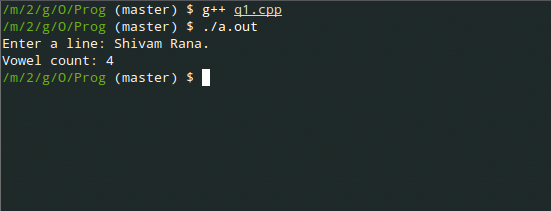
\includegraphics[width=\textwidth]{q1.png}

% Code 2
% \chapter{Number in reverse order}
\section{Number in reverse order}

Print the given number in reverse order. Use functions with return type and without return type for reversing  the number. (eg. 12345 printed as 54321)

\lstinputlisting{q2.cpp}
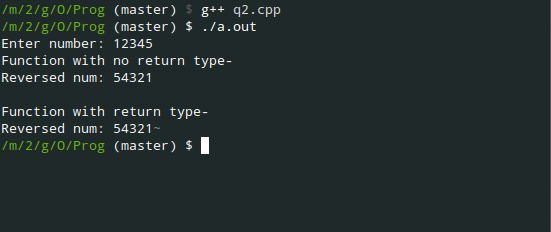
\includegraphics[width=\textwidth]{q2.png}

% Code 3
% \chapter{Arithmetic Operations using Inline Function}
\section{Inline Function}

Program to perform various arithmetic operations such as addition, subtraction, division, modulus, and multiplication using inline function.

\lstinputlisting{q3.cpp}
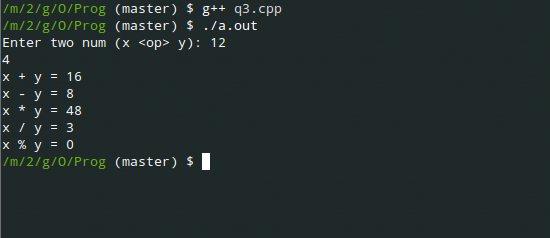
\includegraphics[width=\textwidth]{q3.png}

% Code 4
\chapter{Classes}
\section{Counting the Objects}

Class for counting the number of objects created and destroyed within various block using constructors and destructors.

\lstinputlisting{q4.cpp}
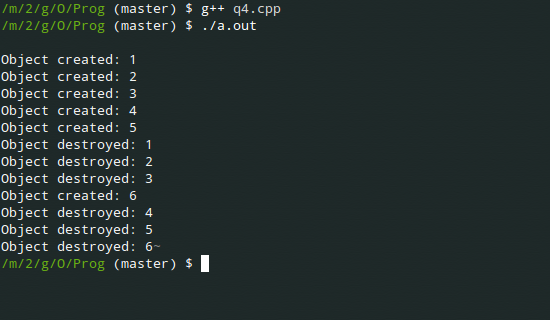
\includegraphics[width=\textwidth]{q4.png}

% Code 5
% \chapter{Classes and 'this' Pointer}
\section{'this' Pointer}

Program to create 3 objects for a class named pntr\_obj with data members such as roll\_no \& name. Create member functions set\_data() for setting the data and print() to print which object has invoked it using 'this' pointer.

\lstinputlisting{q5.cpp}
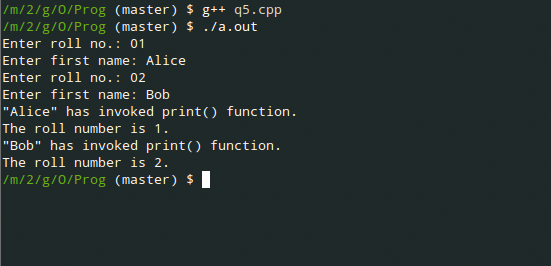
\includegraphics[width=\textwidth]{q5.png}

% Code 6
% \chapter{Virtual Function}
\section{Virtual Function}

Program to implement virtual function (polymorphism) by creating a base class c\_polygon which has virtual function area(). Two classes c\_rectangle and c\_traingle derived from c\_polygon and they have area() to calculate and return the area of rectangle and triangle respectively. 

\lstinputlisting{q6.cpp}
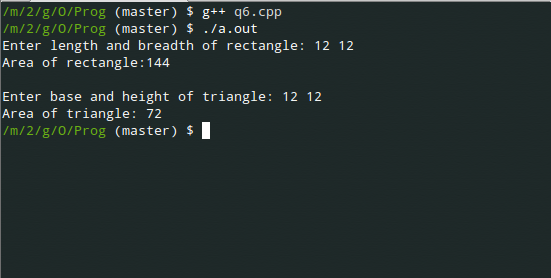
\includegraphics[width=\textwidth]{q6.png}

\chapter{Operator Overloading}

% Code 7
\section{++, - - operators overloaded}

Program to count the number of persons inside a bank, by increasing count whenever a person enters a bank, using an increment (++) operator overloading function, and decrease the count whenever a person leaves the bank using a decrement (- -) operator overloading function inside a class. 

\lstinputlisting{q7.cpp}
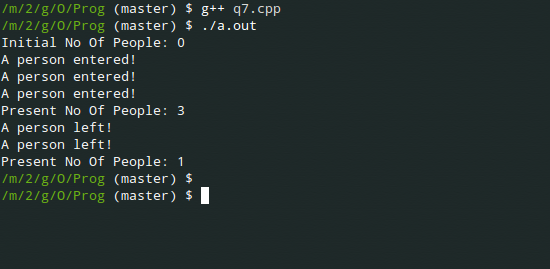
\includegraphics[width=\textwidth]{q7.png}

% Code 8
\section{+, - operators overloaded}

Program to create two objects of a class called company and add their data members using an operator overloaded function for \'+\' operator and \'-\' operator.

\lstinputlisting{q8.cpp}
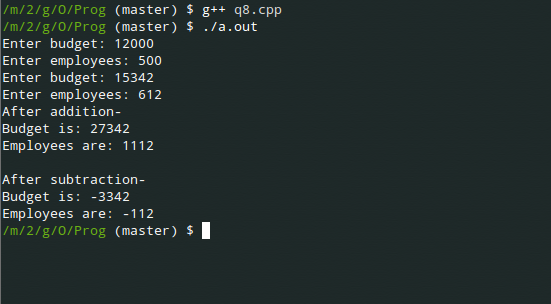
\includegraphics[width=\textwidth]{q8.png}

% Code 9
\section{+, - operators overloaded for matrix Addition and Subtraction}

Create a class matrix and overload +, - operator to perform matrix addition and subtraction.

\lstinputlisting{q9.cpp}
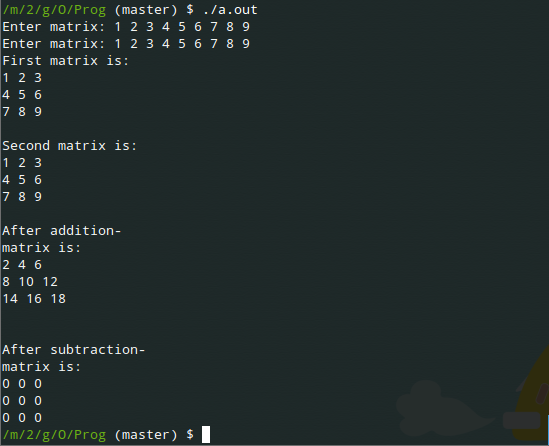
\includegraphics[width=\textwidth]{q9.png}

% Code 14
% \section{Cin and Cout stream operators}

% Overload Cin, Coot stream operators to input and display objects of a class student which contains student details like name, roll no., class, age. 
% Eg: class Student{......}
% Void main()
% {
%     student st;
%     cin>> st;
%     cout<<st;
% }

% \lstinputlisting{q14.cpp}

% Code 10
\chapter{Friends}
\section{Friend Function}

Program to accept five different numbers by creating a class called friendfunc1 and friendfunc2 taking 2 and 3 arg respectively and calculate the average of these numbers by passing object of the class to friend function.

\lstinputlisting{q10.cpp}
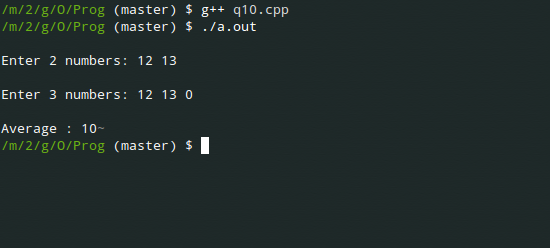
\includegraphics[width=\textwidth]{q10.png}

% Code 11
% \chapter{Friend Class}
\section{Friend Class}

Program to accept the student detail such as name and 3 different marks by get\_data() method and display the name and average of marks using display() method. Define a friend class for calculating the average of marks using the method mark\_avg().

\lstinputlisting{q11.cpp}
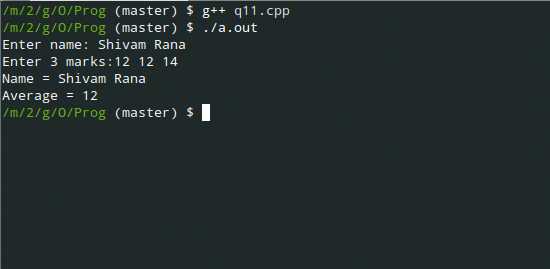
\includegraphics[width=\textwidth]{q11.png}

% Code 12
% \chapter{Template Function called min}

% Program that uses a function template called min to determine the smaller of two arguments. The program should work for integers, characters and floating-point number as arguments to this function.

% \lstinputlisting{q12.cpp}

% Code 13
% \chapter{Class Template}

% Program to explain class template by creating a template T for a class named pair having two data members of type T which are inputted by a constructor and a member function get-max() return the greatest of two numbers to main. Note: the value of T depends upon the data type specified during object creation.

% \lstinputlisting{q13.cpp}

% Code 15
% \chapter{Inheritance}

% Write a class 3D which inherits another class 2D, for 3 dimensional calculations. Using these classes define any 2 points in a 3D space and find the distance between them. The formula for finding the distance between any 2 pts in 3D space is,
% Distance = SquareRoot (xd^2 + yd^2 + zd^2)
% Where, xd = x2 - x1, yd = y2 - y1, y.d = z2 - z1

% \lstinputlisting{q15.cpp}

% Code 16
% \chapter{Calculator in Java with memory concept}

% Program in java to implement a calculator having addition and subtraction operations along with the concept of memory (M+) i.e to store the current value on the screen for later use.

% \lstinputlisting{q16.cpp}

% Code 17
% \chapter{Contact Manager}

% Program that acts as a Contact Manager. It saves the content to a file & retrieves them when asked by the user. Modules of the program include: Add, Delete, Search. Save.

% \lstinputlisting{q17.cpp}

\end{document}
